\documentclass[12pt, oneside]{article}   	% use "amsart" instead of "article" for AMSLaTeX format
%\documentclass[12pt, oneside, draft]{article}   	% use "amsart" instead of "article" for AMSLaTeX format

%%%%%%%%%%%%%%%%%%%%%%%%%%%%%%%%%%%%%%%%%%%%%%%%%
%
% The TexLive distribution is stored in /usr/local/texlive/2020
%
% The definitions of the packages are in /usr/local/texlive/2020/texmf-dist/tex/latex
%
%%%%%%%%%%%%%%%%%%%%%%%%%%%%%%%%%%%%%%%%%%%%%%%%%

\usepackage{xparse}					% Allows for the creation of \NewDocumentCommand shortcuts

\usepackage{geometry}				% See geometry.pdf to learn the layout options. There are lots.
\geometry{letterpaper}				% ... or a4paper or a5paper or ... 
\usepackage[parfill]{parskip}		% Activate to begin paragraphs with an empty line rather than indent
\usepackage{float}					% Float package to exert more control over graphic placement
	
%\usepackage{verbatim}				% Creates a verbatim environment for code / program output
\usepackage{graphicx}				% Use pdf, png, jpg, or eps§ with pdflatex; use eps in DVI mode
									% TeX will automatically convert eps --> pdf in pdflatex
\graphicspath{{./figures/}}         

% Math packages
\usepackage{amssymb}				% Mathematical symbols
\usepackage{amsmath}				% Added for typesetting mathematical formulae
\usepackage{amsthm}					% Added for typesetting mathematical theorems
\usepackage{mathalpha}				% Added for some special characters like Q, Z and N

% Table packages in addition to built in tabular
\usepackage{booktabs}				% Adds extra commands to tabular like \toprule
\usepackage{afterpage}				% For pagination support
\usepackage{longtable}				% Support for longer tables

% Hyperlinks
\usepackage{hyperref}				% For creating internal and HTTP links

% Numbering and references
\numberwithin{equation}{section}          % Number equations within sections
\usepackage[numbers]{natbib}              % For bibliography management

% For Tikz graphics
\usepackage{tikz}					% Package for pgf and TikZ
\usetikzlibrary{shapes,arrows,chains}
\tikzstyle{startstop} = [very thick, rectangle, rounded corners, minimum width=2.5cm, minimum height=0.8cm, text centered, draw=black, text width=2.5cm]
\tikzstyle{action} = [rectangle, rounded corners, minimum width=3cm, minimum height=0.8cm, text centered, draw=black, text width=2.5cm]
\tikzstyle{decision} = [diamond, minimum width=3cm, minimum height=3cm, text centered, draw=black, text width=2cm]
\tikzstyle{arrow} = [thick,->,>=stealth]

% For theorems and definitions - each creates it's own counter which incrementa each use
\theoremstyle{definition}
\newtheorem{proposition}{Proposition}[section]
\newtheorem{define}{Definition}[section]
\newtheorem{axiom}{Axiom}[section]
\newtheorem{theorem}{Theorem}
\newtheorem{lemma}[theorem]{Lemma}
\newtheorem{corollary}[theorem]{Corollary}
\newtheorem*{remark}{Remark}

%SetFonts


\title{On the Asymptotic Density of Convergent Residue Classes in the Collatz Map}
\author{Wayne Brassem}
%\date{}							% Activate to display a given date or no date


\begin{document}

% Document define commands for commonly used items in math mode
\NewDocumentCommand{\setN}{}{\mathbb{N}}				% Set of positive integers, excluding 0
\NewDocumentCommand{\setNo}{}{\mathbb{N}_0}				% Set of positive integers, including 0
\NewDocumentCommand{\setNeven}{}{\mathbb{N}_{even}}		% Set of even positive integers, excluding 0
\NewDocumentCommand{\setNodd}{}{\mathbb{N}_{odd}}		% Set of odd positive integers
\NewDocumentCommand{\setZ}{}{\mathbb{Z}}				% Set of all integers, excluding zero
\NewDocumentCommand{\setZo}{}{\mathbb{Z}_0}				% Set of all integers, including zero
\NewDocumentCommand{\setQ}{}{\mathbb{Q}}				% Set of all rational numbers

% Document define commands for commonly used items not in math mode
\NewDocumentCommand{\Rarr}{}{\textrightarrow{}}			% Right arrow

% Document commands which provide hyperlinks to OEIS sequences referenced herein
\NewDocumentCommand{\OEIS}{m}{\href{https://oeis.org/#1}{#1}}

\maketitle



\begin{abstract}

We study the dynamics of the semi-accelerated Collatz map
\[
g(x) = \begin{cases}
\displaystyle
    \phantom{3x} \frac{x}{2} & \text {if } x \text{ is even}, \\[8pt]
\displaystyle
    \frac{3x+1}{2}           & \text {if } x \text{ is odd}. \\
\end{cases}
\]

For structural analysis we relate $g$ to the fully accelerated map
\[
f(x)=\frac{3x+1}{2^{v_2(3x+1)}}.
\]
Here $v_2(n)$ denotes the 2-adic valuation of $n$ (largest $k$ such that $2^k \mid n$).

Our approach decomposes the positive integers into residue classes determined by
finite parity patterns under the fully accelerated map $f$, which serves as a
symbolic compression of trajectories of the semi-accelerated map $g$. Trajectories
are encoded as parity words (sequences of division counts $v_2(3x+1)$), yielding
associated affine maps that describe the finite-step action of $f$ on entire
classes at once. This framework allows systematic enumeration of convergent residue
classes and quantitative control of their combinatorial growth via a grammar derived
from lower bounds on the total number of divisions by two required for admissibility.

Comparing this growth with the powers of two governing residue-class densities, we
prove that the cumulative natural density of integers belonging to residue classes
with finite stopping time approaches one. Consequently, almost every positive integer
eventually reaches a smaller value under iteration of the map (in the sense of natural
density). While zero-density exceptional trajectories are not excluded, the results
provide a measure-theoretic description of typical Collatz behavior.

\end{abstract}
\newpage


\tableofcontents
\newpage


\section{Introduction}

The $3x+1$ problem, also known as the Collatz conjecture~\cite{Collatz1937}, concerns
the behavior of the map
\[
T(x) =
\begin{cases}
\displaystyle
    \phantom{3x} \frac{x}{2} & \text {if } x \text{ is even}, \\[8pt]
\displaystyle
    3x+1,                    & \text{if $x$ is odd}.
\end{cases}
\]
on the positive integers. It asserts that every positive integer eventually reaches $1$
under iteration of $T$. Despite its elementary formulation, the conjecture has resisted
proof for decades \cite{Lagarias2010,Terras1976}. Extensive computational verification
confirms convergence for all integers up to very large bounds \cite{OliveiraESilva2010},
but such verification does not constitute a proof and offers limited insight into the
global structure of Collatz trajectories.

A useful intermediate form is the \emph{semi-accelerated map}
\[
g(x) = \begin{cases}
\displaystyle
    \phantom{3x} \frac{x}{2} & \text {if } x \text{ is even}, \\[8pt]
\displaystyle
    \frac{3x+1}{2}           & \text {if } x \text{ is odd}. \\
\end{cases}
\]
which applies a single division by two immediately after each odd step. This map preserves
the essential dynamics while simplifying the combinatorial structure of trajectories.

For structural analysis it is convenient to work with the
\emph{fully accelerated map}
\[
f(x)=\frac{3x+1}{2^{v_2(3x+1)}},
\]
defined on odd integers. This map removes all powers of two in a single
iterate and satisfies
\[
f(x)=g^{\,v_2(3x+1)}(x),
\]
where the first iterate applies the odd branch and the remaining iterates are divisions
by two. All symbolic encodings and residue-class constructions in this paper are formulated
in terms of the fully accelerated map.

Our approach is to study the \emph{structural properties} of Collatz trajectories
rather than individual integers. Specifically, we partition the positive integers into
\emph{residue classes} determined by finite sequences of division counts following odd
steps under the fully accelerated map $f$—called \emph{parity words}. Each admissible
parity word corresponds to a finite segment of a trajectory under $f$, terminating at
the first step where the iterate is strictly smaller than its starting value.  

We then associate an \emph{affine map} to each parity word, which compresses the trajectory
segment into a single linear-affine operation that is well-defined modulo a power of two
(formal definition in Section ~\ref{sec:division-counts}). This representation captures the
multiplicative and additive effects of the trajectory while abstracting away the starting
integer, allowing us to reason at the level of classes rather than individual numbers.

To control the growth of the number of convergent classes, we introduce an \emph{increment
grammar} derived from the minimal total number of divisions by two required to produce
admissible parity words. The grammar encodes allowable patterns of growth in these minimal
denominators and underlies a canonical \emph{horizontal-sum construction} for enumerating
all convergent classes (in Section~\ref{sec:increment-grammar}). By comparing the growth rate
of the number of classes with the corresponding powers of two that determine residue-class
density, we develop a framework to rigorously argue (in Section ~\ref{sec:cumulative-density})
that the cumulative density of convergent classes approaches one.

This perspective allows us to prove that almost every positive integer eventually reaches
an iterate strictly smaller than its initial value under iteration of the accelerated map,
in the sense of natural density. While this framework does not exclude the logical possibility
of zero-density exceptional trajectories, it provides a strong quantitative understanding of
typical Collatz dynamics and highlights the combinatorial and arithmetic mechanisms that
govern convergence for the vast majority of integers.

\paragraph{Structure of the Paper.} 
Section~\ref{sec:definitions} introduces stopping time, convergent segments, and residue
classes.   Section~\ref{sec:division-counts} defines parity words, total division counts,
and their associated densities.  Section~\ref{sec:grammar} develops the parity-word grammar
and admissibility conditions, leading to affine representations of residue classes. 
Section~\ref{sec:increment-grammar} presents the increment grammar and horizontal-sum
construction, which enumerates convergent classes and controls their combinatorial growth. 
Section ~\ref{sec:cumulative-density} then applies this machinery to prove the vanishing
density of unconvergent integers and the asymptotic global descent result.


\section{Definitions and Preliminaries}
\label{sec:definitions}

\subsection{Stopping Time}

\begin{define}
The \emph{stopping time} \( \sigma(x) \) of a positive integer \(x\) (sometimes called the finite
stopping time or local descent time) is the minimal integer
\(k \ge 1\) (if such a \(k\) exists) such that
\[
f^k(x) < x.
\]
If no such \(k\) exists, we write \(\sigma(x) = \infty\). Stopping time behavior has been studied
extensively in the context of the $3x+1$ problem \cite{Terras1976}.
\end{define}


\subsection{Convergent Segments}

\begin{define}
A \emph{convergent segment of length \(k\)} is a finite sequence
\[
x, f(x), f^2(x), \ldots, f^k(x)
\]
such that \( f^k(x) < x \) and \(k\) is minimal. No assumption is made about eventual
convergence to 1; only strict descent at step \(k\), i.e., \(k = \sigma(x)\), is required.
Finite segments of this type were considered in the context of the accelerated Collatz map
by Everett \cite{Everett1977}.
\end{define}


\subsection{Residue Classes}

Encoding trajectories via residue classes or arithmetic progressions has appeared in prior
structural approaches to the $3x+1$ problem \cite{Wirsching1998,Chamberland2003}.

\medskip
Iterates are indexed starting from \(0\), so that \(f^0(x)=x\). 
Integers \(x\) and \(y\) are equivalent modulo depth \(k\) if the sequence of parities 
of \(f^i(x)\) and \(f^i(y)\) agree for \(i=0,\dots,k-1\). 
In other words, they share the same parity sequence. 
This convention aligns with
the 0-based combinatorial and OEIS sequences used in the analysis.

\begin{define}[Residue Class of Depth \(k\)]
\label{def:residue-class}
Fix \(k \in \setN\) and \(x \in \setN\). Let $\operatorname{par}(n)=n\bmod 2$.
The \emph{residue class of depth \(k\) with respect to \(f\)} containing \(x\) is
\[
[x]_k := \{ y \in \setN \mid \operatorname{par}(f^i(y)) = \operatorname{par}(f^i(x))
\text{ for } i = 0, 1, \dots, k-1 \}.
\]
\end{define}
Here \([x]_k\) encodes the parity sequence; the associated parity word \(\omega\)
further records the number of divisions by two following each iterates of $f$, as formalized
in Section~\ref{sec:division-counts}.

\begin{remark}[Arithmetic structure]
It will be shown in Section~\ref{sec:grammar} that for each admissible parity word
\(\omega\), the associated residue class \([x]_k\) determined by its induced parity
sequence of depth \(k\), the set \([x]_k\) is either empty or an arithmetic progression
modulo a power of two determined by the total division count \(D(\omega)=d_0+\cdots+d_{m-1}\)
(defined formally in Section~\ref{sec:division-counts}).
\end{remark}

\begin{define}[Convergent Residue Class]
A residue class is called convergent of stopping time $k$ if it satisfies the following properties:
\begin{enumerate}
\item \( f^k(y) < y \) for all \( y \in [x]_k \), and
\item for every \( y \in [x]_k \), no smaller integer \( j < k \) satisfies \( f^j(y) < y \).
\end{enumerate}
Here \(k\) is minimal with this property across the entire class.
The uniformity of stopping time across a class is a consequence of the
fact that all elements share the same parity sequence and hence the same
associated parity word and affine map (Section~\ref{sec:division-counts}).
In Section~\ref{sec:grammar}
we prove that admissible parity words associated to convergent segments generate residue classes
with uniform stopping time.
\end{define}

\begin{remark}
This definition is stronger than requiring \(\sigma(x)=k\) for a single representative
\(x\), since it enforces uniform descent at step \(k\) for all elements of the residue class.
\end{remark}


\section{Division Counts and Path Encoding}
\label{sec:division-counts}

The structure of convergent residue classes is governed by the total number of divisions
by two incurred along an accelerated Collatz trajectory. At each step of the accelerated map
\[
f(x) = \frac{3x+1}{2^{v_2(3x+1)}},
\]
all powers of two are removed from \(3x+1\). The number of removed factors of two at the
\(i\)-th iterate is therefore the 2-adic valuation
\[
d_i := v_2(3 f^i(x) + 1).
\]
Here $d_i$ corresponds to the division count in the transition $f^i(x) \rightarrow f^{i+1}(x)$.
Since the fully accelerated map always produces odd iterates, $3 f^i(x) + 1$ is even and hence
$d_i \ge 1$. 

\begin{lemma}[Uniform Valuation on Residue Classes]
For integers belonging to a fixed residue class determined by a parity word, these
division counts \(d_i\) are identical across the class.
\end{lemma}

\subsection{Formal Definition of Parity Words}

In this section we introduce a symbolic encoding of Collatz trajectories
based on the number of divisions by two removed at each step of the accelerated map.
We call such an encoding a \emph{parity word}. The precise combinatorial
constraints determining which parity words correspond to actual trajectories
are deferred to Section~\ref{sec:grammar}; however, the definitions
given here are sufficient for the analysis of residue class densities.

Let a Collatz path be a sequence of iterates under the accelerated map
\[
f(x) = \frac{3x+1}{2^{v_2(3x+1)}}.
\]

\begin{define}[Parity Word]
A \emph{parity word} of length $m \ge 0$ is a finite sequence
\[
\omega = (d_0, d_1, \dots, d_{m-1}),
\]
where each $d_j$ is a positive integer.  Admissibility constraints on which
sequences can occur are defined in Section~\ref{sec:grammar}.

For $m=0$, the word is empty and represents the \emph{trivial zero-step segment};
it serves as a formal base case in the symbolic and combinatorial constructions
but does not correspond to an odd-step event.
\end{define}

Each parity word formally determines an affine map of any integer $x$:
\begin{equation}
\label{eq:linear-affine-map-m}
x \longmapsto \frac{3^m x + c(\omega)}{2^{d_0+\cdots+d_{m-1}}},
\end{equation}
obtained by symbolic composition of the accelerated map along the word. Here
$c(\omega)$ is a canonical integer uniquely determined by the parity word (see
Appendix~\ref{app:canonical-c}). This representation encodes the arithmetic effect
of the sequence of accelerated steps encoded by the word on any starting integer.

\begin{remark}[Parity Words Encode Structure, Not Values]
Fixing a parity word $\omega$ determines the sequence of arithmetic
operations applied along an accelerated Collatz trajectory. Consequently,
both the linear coefficient $3^m/2^{d_0+\cdots+d_{m-1}}$ and the affine term
$c(\omega)$ depend only on $\omega$ and not on the starting integer.

This allows reasoning about convergence or divergence at the level of
residue classes without reference to specific integers.
\end{remark}

\begin{remark}[Residue Classes and Parity Words]
Each admissible parity word $\omega$ determines a unique arithmetic progression
modulo $2^{D(\omega)}$.
\end{remark}


\subsection{Total Division Count}

Let a parity word $\omega = (d_0, \dots, d_{m-1})$ encode a segment consisting of $m$
iterates of the accelerated map $f$. Each iterate of the fully accelerated map removes
a finite number of factors of two from $3x+1$. This number is precisely the entry of
the parity word corresponding to that iterate.

\begin{define}[Total Division Count]
For a parity word $\omega = (d_0,\dots,d_{m-1})$ encoding the $m$ iterates of $f$
of a path, define its \emph{total division count} by
\[
D(\omega) := \sum_{j=0}^{m-1} d_j,
\]
where $d_j$ equals the 2-adic valuation occurring at the $j$-th iterate for any
trajectory realizing $\omega$.
\end{define}

Thus $D(\omega)$ is precisely the exponent of $2$ appearing in the
denominator of the linear-affine form of the $m$-th iterate of $f$ (see
Equation~\eqref{eq:linear-affine-map-m}).

Parity words with the same length $m$ may differ in the distribution of
divisions by two between steps and hence in their total division count.
However, for each parity word, its total division count $D(\omega)$ is
uniquely determined by the sequence of divisions encoded in the word.

\begin{define}[Minimal Total Division Count]
Let $A020914(m)$ denote the minimal total number of divisions by two among
all \emph{admissible} parity words containing exactly $m$ iterates of $f$.
\end{define}

This quantity is given by $\lceil m \log_2(3) \rceil$, a fact derived in
Section~\ref{sec:grammar} and tabulated in \OEIS{A020914}.  Equivalently,
it is the smallest integer $D$ such that $2^D \ge 3^m$. Intuitively,
each odd step multiplies the trajectory by $3$, so the cumulative divisions
by two must at least balance this growth; hence the minimal total division
count corresponds to the smallest exponent of $2$ that offsets the factor
of $3^m$ in the affine map for a path with $m$ iterates of $f$.


\subsection{Density of Residue Classes}

\begin{lemma}[Disjointness of Residue Classes]
Fix $m \ge 0$. The residue classes induced by distinct parity words
$\omega = (d_0,\dots,d_{m-1})$ with $m$ iterates of $f$ are pairwise disjoint.
\end{lemma}

\begin{proof}
Let $\omega$ be a parity word with $m$ iterates of $f$ and total division count
\[
D(\omega) = \sum_{j=0}^{m-1} d_j.
\]
It determines a affine map
\[
x \longmapsto \frac{3^m x + c(\omega)}{2^{D(\omega)}}.
\]
For the $m$-th iterate of $f$ to be an integer, $x$ must satisfy the
integrality condition
\[
3^m x + c(\omega) \equiv 0 \pmod{2^{D(\omega)}}.
\]
Since $3^m$ is odd, it is invertible modulo $2^{D(\omega)}$, and thus this
congruence determines a unique residue class
\[
x \equiv r_\omega \pmod{2^{D(\omega)}}.
\]

If two distinct parity words $\omega \neq \omega'$ produced the same residue
class, then their integrality conditions would define the same affine map
\[
x \mapsto \frac{3^m x + c}{2^D}.
\]
But the symbolic composition of the accelerated map is unique: at each stage,
the exponent $d_i$ is exactly $v_2(3f^i(x)+1)$, so the sequence of exponents is
uniquely determined by the successive 2-adic valuations along the trajectory,
and hence by the parity word itself. Hence $\omega=\omega'$, a contradiction.
Therefore distinct parity words determine distinct and disjoint residue classes.
\end{proof}

\begin{proposition}
A residue class induced by a parity word $\omega$ has natural density
\[
2^{-D(\omega)}.
\]
In particular, for classes with $m$ iterates of $f$,
\[
\text{density} \le 2^{-A020914(m)}.
\]
\end{proposition}

\begin{proof}
Each residue class is an arithmetic progression with modulus $2^{D(\omega)}$
and exactly one representative per period. The natural density of such a class
is therefore $2^{-D(\omega)}$.
\end{proof}

\begin{remark}
For fixed $m$, there are finitely many admissible parity words with $m$ iterates
of $f$. Let $\widetilde A(m)$ denote the number of such words that correspond to
convergent residue classes. Since the classes are pairwise disjoint, their
total density contribution at iterate depth $m$ is bounded by
\[
\widetilde A(m)\,2^{-A020914(m)}.
\]
\end{remark}


\subsection{Example}

Consider convergent segments with $m=4$ iterates of $f$.  
The minimal total division count for $m=4$ is
\[
A020914(4) = 7.
\]

One admissible parity word attaining this minimum is
\[
\omega = (1,1,1,4),
\]
for which
\[
D(\omega) = 1+1+1+4 = 7.
\]

Composing the accelerated map symbolically yields
\[
f_\omega(x)=\frac{3^4 x + c(\omega)}{2^7}
           = \frac{81x + 65}{128},
\]
so the canonical affine constant for this word is
\[
c(\omega)=65.
\]

The integrality condition
\[
81x + 65 \equiv 0 \pmod{128}
\]
determines a unique residue class
\[
x \equiv 15 \pmod{128}.
\]
Hence all integers in this class have natural density $2^{-7}$.

\medskip

\noindent
\textbf{Interpretation.}
The word $\omega = (1,1,1,4)$ means:

\begin{itemize}
    \item At each of the first three iterates of $f$, $3x+1$ contains exactly one factor of $2$.
    \item At the fourth iterate of $f$, $3x+1$ contains four factors of $2$.
\end{itemize}

Under the accelerated map
\[
f(x)=\frac{3x+1}{2^{v_2(3x+1)}},
\]
all of these divisions occur within a single iterate. Thus $d_3=4$ means that
the fourth iterate divides by $2^4$ in that step. The constant $c(\omega)$ is
fixed entirely by this symbolic structure and ensures that precisely the
integers in the residue class $x \equiv 15 \pmod{128}$ produce integer iterates
under the affine form.

\medskip

This example illustrates that convergence properties depend only on the parity
word $\omega$ and its total division count $D(\omega)$, not on the specific
starting value.


\section{Grammar of Collatz Parity Words}
\label{sec:grammar}

\subsection{Parity Words as Dynamical Encodings}

\begin{remark}[Parity Grammar as a Dynamical Encoding]
Recall from Section~\ref{sec:division-counts} that a \emph{parity word}
$\omega=(d_0,\dots,d_{m-1})$ records the exact 2-adic valuation
$d_i = v_2(3 x_i + 1)$, occurring at each iterate of the fully accelerated
Collatz map.

The parity-word grammar introduced in this section provides a symbolic
encoding of accelerated Collatz dynamics, following the symbolic approach
of Chamberland~\cite{Chamberland2003}. This encoding is not injective:
multiple positive integers can correspond to the same parity word.
Specifically, distinct integers whose trajectories share the same sequence
of division counts after $m$ iterates of the accelerated map $f$ trace the
same parity word, forming the arithmetic residue classes described in
Section~\ref{sec:division-counts}.

Unlike a purely combinatorial encoding, parity words retain essential
dynamical information. Each parity word $\omega=(d_0,\dots,d_{m-1})$
determines the sequence of multiplicative factors of the linear coefficient
\[
r_i = \frac{3}{2^{d_i}},
\]
so that the contractive or expansive contribution of each iterate is
preserved in the linear coefficient (with the affine term handled separately
via $c(\omega)$). This structure will allow us to quantify densities of
residue classes and to formulate sufficient conditions for descent, even
though individual trajectories are collapsed under the encoding.
\end{remark}

\subsection{Admissibility of Parity Words}

\begin{define}[Admissible Parity Word]
\label{def:admissible-parity-word}
Let $\omega = (d_0, \dots, d_{m-1})$ be a parity word and write
$D = d_0+\cdots+d_{m-1}$. Associated to $\omega$ is the affine map
\[
F_\omega(x) = \frac{3^m x + c(\omega)}{2^{D}},
\]
where $c(\omega)$ is the canonical integer determined by $\omega$.

The parity word $\omega$ is said to be \emph{admissible} if there exists at
least one integer $x$ such that $F_\omega(x)$ is an integer. Equivalently,
$\omega$ is admissible if the numerator $3^m x + c(\omega)$ is divisible by
$2^{D}$ for at least one residue class of $x \bmod 2^{D}$.
\end{define}

\begin{remark}
Admissibility is therefore an arithmetic condition on the word $\omega$
itself, expressed as a divisibility constraint on the associated affine
map. When this condition holds, the set of all integers $x$ for which
$F_\omega(x)$ is integral forms a unique residue class modulo $2^{D}$,
corresponding to the residue class induced by $\omega$.
\end{remark}

\begin{lemma}[Minimal Division Count]
For any admissible parity word $\omega=(d_0,\dots,d_{m-1})$ of length $m$,
\[
d_0 + \cdots + d_{m-1} \;\ge\; A020914(m),
\]
where
\[
A020914(m) = \lceil m \log_2(3) \rceil.
\]
Equality holds if and only if $\omega$ achieves the minimal possible total
division count among admissible words of length $m$.
\end{lemma}

\begin{define}[Convergent Parity Word]
An admissible parity word $\omega = (d_0,\dots,d_{m-1})$ is said to be
\emph{convergent} if
\[
\frac{3^m}{2^{d_0+\cdots+d_{m-1}}} < 1.
\]
\end{define}

\begin{remark}[Role of the Affine Term]
The constant term $c(\omega)$ in the affine representation
\[
F_\omega(x) = \frac{3^m x + c(\omega)}{2^{d_0+\cdots+d_{m-1}}}
\]
encodes the cumulative effect of the additive term inherited from the classical
$3x+1$ map along the trajectory determined by $\omega$. Admissibility ensures
that this affine map corresponds to genuine Collatz dynamics, mapping a nonempty
arithmetic progression of integers to integers. Once admissibility is established,
the condition
\[
\frac{3^m}{2^{d_0+\cdots+d_{m-1}}} < 1
\]
characterizes the asymptotic behavior of the map: the associated linear factor
is \emph{contractive}. Thus, although the additive term affects the finite-scale
behavior of individual trajectories, the criterion for convergence depends only
on the multiplicative component of the affine map.
\end{remark}


\subsection{Residue Classes Induced by Parity Words}

Fix a parity word $\omega = (d_0,\dots,d_{m-1})$ of length $m$ that is
admissible in the sense of Definition~\ref{def:admissible-parity-word}.
Let
\[
D(\omega) := d_0 + \cdots + d_{m-1}
\]
denote its total division count. By admissibility,
$D(\omega) \ge A020914(m)$.

\begin{lemma}[Residue Class Modulus]
\label{lem:residue-modulus}
Let $x,y \in \setN$ both realize the same parity word $\omega$, i.e.,
their trajectories under $f$ exhibit the division counts encoded by $\omega$
for the first $m$ iterates of the accelerated map $f$. Then
\[
x \equiv y \pmod{2^{D(\omega)}}.
\]
\end{lemma}

\begin{proof}
For any integer $z$ realizing $\omega$, the $m$ iterates of the accelerated map
$f$ encoded by $\omega$ induce the affine relation
\[
F_\omega(z) = \frac{3^m z + c(\omega)}{2^{D(\omega)}},
\]
where $F_\omega(z)\in\setN$ by admissibility.
Thus $3^m z + c(\omega)$ is divisible by $2^{D(\omega)}$.

If both $x$ and $y$ realize $\omega$, then
\[
3^m x + c(\omega) \equiv 0 \equiv 3^m y + c(\omega) \pmod{2^{D(\omega)}},
\]
which implies
\[
3^m(x-y) \equiv 0 \pmod{2^{D(\omega)}}.
\]
Since $3^m$ is invertible modulo $2^{D(\omega)}$, it follows that
\[
x \equiv y \pmod{2^{D(\omega)}}.
\]
\end{proof}

\begin{lemma}[Associated Affine Collatz Map]
\label{lem:associated-map}
Each admissible parity word $\omega$ induces a unique affine map
\[
F_\omega(x) = \frac{3^m x + c(\omega)}{2^{D(\omega)}},
\]
where $c(\omega)$ is uniquely determined modulo $2^{D(\omega)}$ by the
requirement that $F_\omega(x)\in\setN$ for all integers $x$ in the residue class
induced by $\omega$.
\end{lemma}

\begin{remark}[Affine Compression of Trajectories]
For any integer realizing a parity word $\omega$, the value $F_\omega(x)$
coincides exactly with the result of applying the accelerated Collatz map
through the $m$ iterates of the accelerated map $f$ encoded by $\omega$,
including all intermediate divisions by two. Thus $F_\omega$ represents a
compression of a finite Collatz trajectory into a single affine step.
\end{remark}

\begin{lemma}[Convergent Residue Class]
\label{lem:residue-class}
Each convergent parity word $\omega$ induces a unique arithmetic residue class
\[
x \equiv r_\omega \pmod{2^{D(\omega)}},
\]
whose elements all follow the same parity pattern for $m$ iterates of the
accelerated map $f$ and satisfy
\[
F_\omega(x) < x.
\]
for all
\[
x > \frac{c(\omega)}{2^{D(\omega)} - 3^m}.
\]

Consequently, every element of the class reaches a strictly smaller integer
after completing the $m$ iterates of the accelerated map $f$ encoded by $\omega$.
\end{lemma}


\section{Increment Grammar and Horizontal-Sum Construction}
\label{sec:increment-grammar}

\begin{remark}[Increment Grammar from Minimal Denominator Growth]
The first difference sequence of $A020914$, given by \OEIS{A022921},
induces a binary \emph{increment grammar} $\{s,d\}$ that describes the growth
of the \emph{minimal admissible} total division count as the number of odd steps increases.

Each symbol records whether the minimal total division count increases by one ($s$) or
two ($d$) when extending an admissible word by one additional odd step. Importantly, this
grammar \emph{does not} encode the realized parity word entries $d_i$ (which may be arbitrarily
large), but rather governs the evolution of the minimal denominator required for admissibility.

The increment grammar underlies the \emph{horizontal-sum construction} used to enumerate
all convergent parity words, admitting a canonical tabular realization. Specifically, admissible
local patterns within the $\{s,d\}$ grammar determine the combinatorial growth of $\widetilde A(m)$
independently of the particular values of the parity word entries.
\end{remark}

\begin{proposition}
The number of convergent parity words of length $m$ is given by \OEIS{A186009}.
\end{proposition}

\begin{remark}[Canonical Tabular Realization]
A canonical realization of this counting sequence via the horizontal-sum construction,
together with its derivation from the increment grammar induced by \OEIS{A022921}, is given
in Appendix~\ref{app:horizontal-sum-table}. The appendix serves as a structural reference:
the arguments in this section rely only on the grammar itself and not on any numerical
properties of the tabulation.
\end{remark}

\begin{lemma}[Single-to-Double Row Sum Bound]
\label{lem:single-double-bound}
Consider a row produced by a \emph{single} increment step with total sum $S$ (i.e., the
sum of its entries in the horizontal-sum table). If a \emph{double} increment is applied
immediately afterward, the resulting row has total less than $3S$.
\end{lemma}

\begin{proof}
By definition, the total sum of the single row equals $S$.  Under a subsequent double step,
the terminal entry of the new row is formed as the sum of all entries of the preceding row,
and the previous terminal entry is duplicated.

Since the terminal entry of every row is the sum of the preceding row and is therefore 
strictly positive, the interior entries constitute a proper subset of the row’s mass, and
their total is strictly less than $S$.

Thus the double row consists of:
\begin{enumerate}
    \item The interior entries of the single row, whose total is $S_{\rm int} < S$;
    \item One terminal entry equal to $S$; and
    \item A duplicated terminal entry, also equal to $S$.
\end{enumerate}

Hence the total sum of the double row is bounded by
\[
S_{\rm int} + S + S < 3S.
\]
\end{proof}

\begin{remark}[Controlled Maximal Growth]
This lemma ensures that doubling steps contribute at most a controlled multiplicative
factor to horizontal-sum growth, independent of the global cycle structure. Consequently,
all admissible local patterns within a finite cycle admit finite maximal growth factors,
which can be explicitly enumerated (see Appendix~\ref{app:local-growth-details}).  
These bounds are key to establishing the vanishing density of residue classes
associated with increasingly long stopping times.
\end{remark}


\section{Cumulative Density of Convergent Classes}
\label{sec:cumulative-density}

\begin{remark}[Roadmap]
In this section we combine the constructions developed in Sections~\ref{sec:grammar}
and~\ref{sec:increment-grammar} to analyze the asymptotic density of convergent residue
classes. First, we record the number of admissible residue classes of stopping time
\(i\) via the sequence \(\widetilde A(i) = A186009(i+1)\) and the associated minimal
denominator growth \(B(i) = A020914(i)\). Then, using uniform bounds on \(2^{B(i)}\)
and the grammar-enforced suppression of locally expansive horizontal-sum growth, we show
that the per-step growth of \(\widetilde A(i)\) is strictly dominated by the denominator.
Finally, this establishes that the density contribution of newly appearing convergent
residue classes vanishes as \(i\to\infty\), implying that almost every positive integer
belongs to at least one convergent residue class.
\end{remark}


\subsection{Density Contributions and Denominator Growth}

Define
\[
\widetilde A(i) := A186009(i+1),
\]
so that $\widetilde A(i)$ counts convergent residue classes of stopping time $i$.

Let
\[
B(i) := A020914(i),
\]
so that the density contribution of convergent residue classes of stopping time $i$ is
\[
\widetilde A(i)\, 2^{-B(i)}.
\]

By definition of $A020914$ as the minimal exponent with $2^{B(i)} > 3^i$, the function
$B(i)$ satisfies the following properties:
\begin{itemize}
    \item $B(i)$ is strictly increasing, with increments either 1 or 2 (never zero).
    \item By construction, $2^{B(i)} > 3^i$ for all $i \ge 0$.
    \item Consecutive powers of two differ by a factor of 2, so
    \[
    3^i < 2^{B(i)} < 2 \cdot 3^i.
    \]
\end{itemize}

Because $B(i)$ is defined as the minimal integer with $2^{B(i)} > 3^i$,
the quantity $2^{B(i)}$ is the smallest power of two exceeding $3^i$.
Since consecutive powers of two differ by a factor of $2$, we obtain the sharp bound
\[
3^i < 2^{B(i)} < 2 \cdot 3^i \quad \text{where } B(i) = A020914(i).
\]

\begin{remark}[Indexing and Effective Growth Delay]
The OEIS sequences \(A020914\) and \(A186009\) employ differing indexing
conventions. In order to compare numerator and denominator growth on a common
scale, we define \(\widetilde A(i) := A186009(i+1)\), so that the index \(i\)
corresponds uniformly to stopping time (equivalently, parity-word length).

While the first doubling increment in $A020914$ occurs at index $1$, its
effect on $\widetilde A$ appears after a fixed finite delay of two growth
steps. This delay is independent of $i$ and does not affect the asymptotic
growth comparison between numerator and denominator, which is controlled by
the increment grammar introduced in Section~\ref{sec:increment-grammar}.
\end{remark}

\noindent
\textbf{Constant-factor control.}
This bound depends only on the definition of $A020914$ and does not rely on
any delayed-doubling or numerator-growth arguments. Consequently, the reciprocal satisfies
\[
2^{-B(i)} \in \left( \frac{1}{2 \cdot 3^i}, \frac{1}{3^i} \right),
\]
providing a \emph{uniform constant-factor bound} for the density contribution at stopping time $i$.

We now record this observation formally, as it provides the fixed exponential scale against
which numerator growth will be compared.

\begin{lemma}[Uniform Control of Density Contributions]
\label{lem:uniform-control}
For all $i \ge 0$,
\[
3^i < 2^{A020914(i)} < 2\cdot 3^i.
\]
Consequently, the density contribution of convergent residue classes of
stopping time $i$, given by \(\widetilde A(i) 2^{-A020914(i)}\), satisfies
\[
\frac{\widetilde A(i)}{2 \cdot 3^i}
\;<\;
\widetilde A(i)\,2^{-A020914(i)}
\;<\;
\frac{\widetilde A(i)}{3^i}.
\]
\end{lemma}

\begin{proof}
By definition, $A020914(i)$ is the minimal integer $m$ such that $2^m > 3^i$.
Consecutive powers of two differ by a factor of $2$, so
\[
3^i < 2^{A020914(i)} < 2 \cdot 3^i.
\]
Taking reciprocals and multiplying by $\widetilde A(i)$ gives the stated bounds.
\end{proof}


\subsection{Growth Rate of the Number of Convergent Classes}

\begin{remark}[Grammar-Enforced Suppression of Expansive Growth]
\label{rem:grammar-suppression}
The proof of Theorem~\ref{thm:maximal-growth} does not rely on the absence of
locally expansive configurations. Certain increment patterns are expansive in isolation,
but the increment grammar forbids them or requires surrounding contractive structure.

\medskip
\noindent\textbf{(1) Local expansivity versus admissibility.}
A single double increment $\{d\}$ or the short pattern $\{s,d,d\}$ produces
horizontal-sum growth with geometric mean exceeding $1$. However, neither pattern
is admissible under the increment grammar induced by \OEIS{A022921}, as all admissible
sequences must begin with $\{s\}$ and no occurrence of $\{d,d\}$ may appear without
sufficient separating structure.

\medskip
\noindent\textbf{(2) Minimal realization of expansion.}
The shortest admissible pattern containing a double increment $dd$ is
the length-$5$ block
\[
\{s,d,s,d,d\},
\]
which constitutes the minimal expansive configuration. All admissible patterns
of length $\le 4$ are contractive.

\medskip
\noindent\textbf{(3) Forced contractive buffering.}
The grammar enforces that the expansive $5$-cycle cannot appear in isolation. 
The minimal admissible prefix leading to a $\{d,d\}$ occurrence is the length-$7$
block
\[
\{s,d,s,d,s,d,d\},
\]
which is contractive. Concatenating the expansive $5$-cycle with this prefix yields
a length-$12$ block that is also contractive. Thus expansive behavior is always
dominated by mandatory contractive buffers.

\medskip
\noindent\textbf{(4) Consequence for asymptotic growth.}
Any admissible infinite increment sequence decomposes into finite grammar-allowed
blocks. Horizontal-sum growth is submultiplicative under concatenation, so the
asymptotic per-step growth rate is bounded above by the largest geometric mean
among admissible blocks. Expansive blocks are separated by uniformly bounded
contractive buffers, ensuring their asymptotic density in any admissible sequence
is strictly less than one.
\end{remark}

\begin{theorem}[Maximal Admissible Growth Rate for $\widetilde A = A186009$]
\label{thm:maximal-growth}
Let $\widetilde A(i) = A186009(i+1)$ denote the number of convergent residue classes
of stopping time $i$, generated by the horizontal-sum construction associated with
the increment grammar of \OEIS{A022921}.  Let $B(i) := A020914(i)$ denote the
cumulative exponent of $2$ up to level $i$.  

Then the per-step growth of $\widetilde A(i)$ is bounded by the maximal geometric growth
rate of a $5$--cycle (see Appendix~\ref{app:local-growth-details}, Equation~\eqref{eq:rho-5}):
\[
\limsup_{i\to\infty} \widetilde A(i)^{1/i} \le \rho_5 < 3,
\]
and consequently
\[
\frac{\widetilde A(i)}{2^{B(i)}} \;\longrightarrow\; 0 \quad \text{as } i\to\infty.
\]
\end{theorem}

\begin{proof}
The increment sequence \OEIS{A022921} induces a finite symbolic grammar on $\{s,d\}$,
corresponding to single and double increments in the horizontal-sum construction.

Among all admissible sequences, the shortest potentially expansive configuration is the
\emph{5-cycle}
\[
\{s,d,s,d,d\}.
\]
All admissible words of length $\le 4$ produce horizontal-sum growth factors with
geometric mean $\le 1$. A complete enumeration of admissible local patterns and
their growth factors is given in Appendix~\ref{app:local-growth-details}.

Explicit computation of the net growth factor for the 5-cycle gives
\[
\rho_5 := \bigl(\text{total sum after 5-cycle}\bigr)^{1/5} < 3.
\]

Any admissible infinite increment sequence decomposes into concatenations of finite
blocks permitted by the grammar. As explained in Remark~\ref{rem:grammar-suppression},
all locally expansive blocks are separated by mandatory contractive buffering. Horizontal-sum
growth is submultiplicative under concatenation, so the asymptotic per-step geometric
growth is bounded above by the maximal geometric mean among admissible blocks, which is
attained by the $5$-cycle and denoted $\rho_5$. Hence
\[
\limsup_{i\to\infty} \widetilde A(i)^{1/i} \le \rho_5 < 3.
\]

From Lemma~\ref{lem:uniform-control}, the denominator satisfies
\[
3^i < 2^{B(i)} < 2\cdot 3^i.
\]
Consequently, there exists a constant $C>0$, depending only on initial conditions
and finite prefixes, such that
\[
\widetilde A(i) \le C\,\rho_5^i \quad \text{for all } i.
\]
Dividing by $2^{B(i)}$ gives
\[
\frac{\widetilde A(i)}{2^{B(i)}} \le \frac{C\,\rho_5^i}{3^i} \longrightarrow 0,
\]
which completes the proof.
\end{proof}


\subsection{Vanishing of the Cumulative Density}

The preceding results show that although the number of convergent residue classes
$\widetilde A(i)$ grows with stopping time, its growth rate is strictly dominated
by the denominator $2^{B(i)}$, which grows asymptotically like $3^i$.

By Lemma~\ref{lem:uniform-control}, the density contribution at level $i$ satisfies
\[
\frac{\widetilde A(i)}{2 \cdot 3^i} < \widetilde A(i)\,2^{-B(i)} < \frac{\widetilde A(i)}{3^i}.
\]

By Theorem~\ref{thm:maximal-growth}, we have
\[
\frac{\widetilde A(i)}{3^i} \longrightarrow 0 \quad \text{as } i\to\infty.
\]
Hence, the density contribution of newly appearing convergent residue classes at stopping
time $i$ tends to zero as $i \to \infty$.

Consequently, for any fixed \(\epsilon>0\), there exists an \(i_0\) such that the
total density contribution of all convergent residue classes appearing after stopping
time \(i_0\) is less than \(\epsilon\). In other words, the set of positive integers
that fail to belong to any convergent residue class has asymptotic density zero.
Equivalently, almost every positive integer lies in at least one convergent residue
class with respect to natural density, showing that convergent behavior dominates
the Collatz map in a measure-theoretic sense.

\paragraph{Remark on growth bounds.}
The preceding argument is purely measure-theoretic and does not rely on lower
bounds for the growth of \(\widetilde A(i)\). Nevertheless, it is possible to
establish a nontrivial exponential lower bound on the growth rate of
\(\widetilde A(i)\) by comparison with the auxiliary sequence \OEIS{A047749},
which admits a closed-form binomial representation. This comparison shows that
the exponential growth rate of \(\widetilde A(i)\) is bounded below by
\(\sqrt{27/4}\). The derivation of this bound is independent of the density
argument and is developed separately in Appendix~\ref{app:A047749-lower-bound}.


\section{Global Descent in Density}

\begin{theorem}[Asymptotic Global Descent]
\label{thm:asymptotic-descent}
The union of convergent residue classes has asymptotic density one. Consequently,
almost every positive integer eventually reaches a smaller value under iteration
of the accelerated Collatz map, in the sense of natural density.
\end{theorem}

\begin{proof}
Let $\widetilde A(i) = A186009(i+1)$ denote the number of convergent residue classes
of stopping time $i$, and let $B(i) = A020914(i)$ denote the cumulative exponent
of $2$ at level $i$. By Theorem~\ref{thm:maximal-growth}, we have
\[
\frac{\widetilde A(i)}{2^{B(i)}} \longrightarrow 0 \quad \text{as } i \to \infty.
\]

By construction, each residue class consists of integers that descend after finitely many
odd-step iterations. Since the total density of all convergent residue classes approaches
one, the set of integers not contained in any convergent residue class has asymptotic
density zero.  

Therefore, for almost every positive integer $x$ (in the sense of natural density),
there exists a finite $k$ such that
\[
f^k(x) < x,
\]
where $f$ denotes the accelerated Collatz map.
\end{proof}

\begin{remark}[Exceptional Orbits]
This theorem does not preclude the existence of exceptional trajectories outside
the convergent residue classes. Any such set must have asymptotic density zero, 
so the result establishes descent in a measure-theoretic sense rather than an absolute guarantee.
\end{remark}


\section{Consequences for Hypothetical Zero-Density Exceptional Trajectories}

The density result established above does not exclude the logical possibility of
non-convergent Collatz trajectories. However, it severely restricts the form that
any such trajectory could take. In particular, any exceptional set must lie entirely
outside the union of convergent residue classes whose cumulative asymptotic density
approaches one, confining any hypothetical exception to a set of asymptotic density zero.

Consequently, an exceptional trajectory could not belong to any of the residue-class
families constructed in the preceding sections, nor arise from the structured parity
patterns that generate those classes. Any trajectory avoiding all convergent residue
classes would also avoid all patterns admissible under the increment grammar, highlighting
the structural rigidity imposed by the combinatorial framework.

In this sense, any hypothetical exception would be \emph{dynamically isolated}: it would
not be supported by a scalable arithmetic structure or by a residue-class hierarchy of
positive density, but would instead persist only as a sparse, non-propagating phenomenon
within the integer space.


\section{Conclusion}

In this work, we have analyzed the Collatz map via a structural decomposition
of the positive integers into non-overlapping residue classes determined by
finite parity patterns, each associated with a minimal stopping time. By enumerating
convergent parity words and controlling the maximal admissible growth rate relative
to the corresponding powers of two, we rigorously demonstrated that the cumulative
density of convergent classes approaches one.

This density-based approach establishes that almost every positive integer eventually
reaches a strictly smaller value under the accelerated Collatz map. While the argument
does not preclude zero-density exceptional trajectories, it provides a strong
measure-theoretic framework for understanding the typical dynamics of the map.

Viewed abstractly, this perspective reframes the Collatz problem as an analysis of
integer lattices partitioned by arithmetic residue classes, highlighting how parity-
and residue-based combinatorial structures govern discrete dynamical systems. It
emphasizes the distinction between “almost all” and “all,” yielding a credible,
rigorous statement fully consistent with the density analysis.


\newpage
\appendix
\section{Canonical Determination of the Constant \(c(\omega)\)}
\label{app:canonical-c}

Each parity word \(\omega\) induces an affine map \(F_\omega(x)\) of length $m$
(see Section~\ref{sec:division-counts})
\[
F_\omega(x) = \frac{3^m x + c(\omega)}{2^D}, \qquad D = d_0 + \dots + d_{m-1},
\]
where \(c(\omega)\) is uniquely defined modulo \(2^D\). In this appendix,
we describe a canonical choice and a simple method to compute it.

\subsection*{Canonical Choice}

For a fixed \(\omega\), any integer \(x\) in the corresponding residue class satisfies
\[
3^m x + c \equiv 0 \pmod{2^D}.
\]
We remove ambiguity by selecting the unique representative
\[
0 \le c(\omega) < 2^D.
\]
This choice depends only on \(\omega\) and is independent of the representative \(x\).

\subsection*{Step-by-Step Computation}

Given \(\omega\) of length \(m\) and total division count \(D\):

\begin{enumerate}
\item Choose any integer \(x\) in the residue class corresponding to \(\omega\).  
\item Compute \(y = 3^m x\).  
\item Let \(r = \lceil y / 2^D \rceil\) be the smallest integer such that \(r \cdot 2^D \ge y\).  
\item Define \(c(\omega) = r \cdot 2^D - y\).  
\end{enumerate}

By this construction, \(0 \le c(\omega) < 2^D\) ensuring that
\[
F_\omega(x) = \frac{3^m x + c(\omega)}{2^D} \in \mathbb{Z} \quad \text{for all } x \text{ in the class.}
\]

\newpage
\subsection*{Example}

Let \(\omega = (1,1,1,4)\) with \(m=4\) and \(D = \sum_{i=0}^{3} d_i = 1 + 1 + 1 + 4 = 7\):

\begin{enumerate}
\item Choose \(x = 15\). Compute \(y = 3^4 \cdot 15 = 1215\).  
\item \(2^7 = 128\), so \(r = \lceil 1215/128 \rceil = 10\).  
\item \(c(\omega) = 10 \cdot 128 - 1215 = 65\).  
\end{enumerate}

Hence the canonical map is
\[
F_\omega(x) = \frac{81x + 65}{128}.
\]

Checking another representative \(x = 143\):
\[
F_\omega(143) = \frac{81 \cdot 143 + 65}{128} = 91,
\]
confirming that the same \(c(\omega)\) works for the entire residue class.

\subsection*{Remark}

This construction is purely illustrative and is not required for the density
or extremal growth arguments in the main text. It demonstrates concretely
how the affine map is fully determined by the parity word \(\omega\).


\newpage
\section{Extremal Local Growth Analysis}

\begin{lemma}[Local Growth Bounds]
\label{lem:local-growth-bounds}

For each admissible local pattern occurring within \OEIS{A022921},
the ratio of the total sum of entries after applying the pattern
to the total sum before applying it is bounded above as follows,
uniformly over all admissible placements of (delayed) doubling within
the pattern:
\[
\begin{array}{c|c}
\text{Pattern} & \text{Max Growth Factor} \\
\hline
s,d & 3 \\
d,d & 123/33 \\
s,d,s & 341/131 \\
d,d,s & 329/123
\end{array}
\]
Here $s$ denotes a single increment and $d$ a double increment in the
horizontal-sum construction.
\end{lemma}

\begin{proposition}[Extremal 5-Cycle Growth]
\label{prop:extremal-5-cycle}
The maximal geometric growth rate achievable by any admissible infinite
word under the horizontal-sum dynamics associated with \OEIS{A186009} is bounded by
\[
\rho_{5}
=
\Bigl(
3^{2}
\cdot (123/33)^1
\cdot (341/131)^1
\cdot (329/123)^1
\Bigr)^{1/5}
\approx 2.95
< 3,
\]
where the exponents count the occurrences of each local pattern within a $5$-cycle, which
is the minimal admissible expansive block (see Remark~\ref{rem:grammar-suppression}).
\end{proposition}

\noindent
Here the exponents record the total number of coefficients generated by each
admissible local pattern within a single $5$--cycle; the enumeration of these
patterns and the derivation of the exponents $2,1,1,1$ are given explicitly in
Appendix~\ref{app:local-growth-details}, Section~\ref{sec:admissible-patterns}.

\begin{remark}[Connection to Theorem~\ref{thm:maximal-growth}]
The quantity \(\rho_5\) defined above is precisely the maximal geometric growth rate
used in Theorem~\ref{thm:maximal-growth} to bound
\(\limsup_{i\to\infty} \widetilde A(i)^{1/i}\). This establishes that, asymptotically,
the number of convergent residue classes grows strictly slower than the corresponding
powers of two, ensuring vanishing density for large stopping times.
\end{remark}

\begin{remark}[Derivation and Attribution of Local Growth Constants]
The horizontal-sum framework used to analyze $\widetilde A(i)$ is inspired by
the Pascal-type summation approach introduced by Winkler~\cite{Winkler2017},
which provided the original insight that admissible Collatz parity words can
be organized into structured combinatorial growth processes. The present work
adapts this perspective to the specific setting of \OEIS{A022921} and
\OEIS{A186009}, and extends it by performing an explicit extremal analysis of
local growth configurations.

The constants shown in Lemma~\ref{lem:local-growth-bounds} are obtained by
examining the horizontal-sum dynamics governing $\widetilde A(i)$.
Within each local configuration, elements arising from single steps evolve
according to standard Pascal-type summation, yielding maximal growth
proportional to powers of $2$. Additional entries introduced by doubling steps
are bounded by summing on top of this baseline growth.

For each admissible local pattern occurring within \OEIS{A022921}, all possible
placements of delayed doubling contributions were examined, and the largest
achievable ratio of post-pattern to pre-pattern row sums was recorded. No
assumptions beyond the combinatorial structure of the horizontal-sum
construction are used.

A complete derivation of the horizontal-sum mechanism, together with detailed
computations of all local growth constants and their admissible concatenations,
is given in Appendix~\ref{app:local-growth-details}. Consequently, while the
conceptual framework traces back to Winkler’s original insight, the bounds
employed here are established entirely within the present paper.

It follows that any admissible sequence under \OEIS{A022921}, including those
relevant for \OEIS{A186009}, is strictly dominated in per-symbol growth by a
concatenation of $5$-cycles, yielding the uniform bound of
Proposition~\ref{prop:extremal-5-cycle}.
\end{remark}


\newpage
\section{Extremal Local Growth Calculations}
\label{app:local-growth-details}

Recall that the sequence \OEIS{A020914} has first differences given by
\OEIS{A022921}, consisting of repeated blocks of \emph{single} steps ($s$) and \emph{double} steps ($d$).

\subsection{Cycle Structure and Net Multiplicative Effect}

A frequently occurring block is the $7$--cycle
\[
\{ s, d, s, d, s, d, d \},
\]
which contains $3$ singles and $4$ doubles.  The corresponding number of
factors of $2$ is
\[
3 + 2(4) = 11,
\]
so the net multiplicative contribution of this cycle satisfies
\[
\frac{2^{11}}{3^7} < 1.
\]

Thus the $7$--cycle is strictly contractive. Every $7$--cycle is followed by a $5$--cycle
\[
\{ s, d, s, d, d \},
\]
which contains $2$ singles and $3$ doubles, contributing
\[
2 + 2(3) = 8
\]
factors of $2$.  Since
\[
\frac{2^8}{3^5} > 1,
\]
the $5$--cycle is expansive.

Concatenating the $7$--cycle and $5$--cycle produces a $12$--cycle
\[
\{ s, d, s, d, s, d, d, s, d, s, d, d \},
\]
containing $5$ singles and $7$ doubles.  The total number of factors of $2$ is
\[
5 + 2(7) = 19,
\]
and hence
\[
\frac{2^{19}}{3^{12}} < 1.
\]
Therefore, the $12$--cycle is again contractive.

Repeated 12-cycles remain contractive, suppressing growth until enough
slack accumulates to allow a 5-cycle insertion. The 5-cycle represents the
unique locally expansive pattern, though its repetition is constrained by
the grammar.

\subsection*{Horizontal-Sum Dynamics and Pascal-Type Growth}

The generating rows evolve by a horizontal-sum rule:
\begin{equation}
a_i(n) = a_i(n-1) + a_{i-1}(n), \quad i,n \in \mathbb{N},
\label{eq:horizontal-sum-recurrence}
\end{equation}
so that sequences of single steps exhibit ordinary Pascal--type growth.
Double steps differ in that the terminal entry is duplicated, causing the
final term to appear twice while preserving monotonicity.

Because the grammar forces expansive configurations to appear only within this minimal 5-block,
extremal asymptotic growth is realized by repeated alignment of this block, making it sufficient
to analyze this configuration.  Thus for extremal 5-cycle analysis, the local maximal sequence
(dominating per-pattern growth) is
\[
\{ s, d, s, d, d \}, \{ s, d, s, d, d \},
\]
enumerating occurrences of each admissible local pattern within a 5-cycle.

\subsection*{Admissible Local Patterns}
\label{sec:admissible-patterns}

Within \OEIS{A022921}, only four local configurations occur:
\[
(s, d), \quad (d, d), \quad (s, d, s), \quad (d, d, s).
\]

The associated coefficient counts within a 5-cycle are:
\[
\begin{array}{c|c}
\text{Pattern} & \text{Associated coefficient count} \\
\hline
s,d & 2 \\
d,d & 1 \\
s,d,s & 1 \\
d,d,s & 1
\end{array}
\]

\subsection{Illustrative Extremal Computations}

The generating rows evolve by a horizontal--sum rule:
\[
a_{i}(n) = a_i(n-1) + a_{i-1}(n); i,n \in \setN,
\]
so that sequences of single steps exhibit ordinary Pascal--type growth.
Double steps differ only in that the terminal entry of the row is duplicated,
causing the final term to appear twice in the generating tuple while preserving
monotonicity of the preceding entries.

% These examples are representative extremal probes of the recurrence.  Since
% Lemma~\ref{lem:single-double-bound} provides uniform inequalities valid for all
% admissible generating rows, any realization saturating these inequalities
% yields an upper bound on every occurrence of the same local pattern.

These examples are chosen so that each step saturates the inequalities of
Lemma~\ref{lem:single-double-bound}, thereby realizing extremal growth. Equalities
shown below should be interpreted as extremal upper-bound realizations rather than
identities valid for all rows.

Let $S$ denote the total sum of entries in the generating row prior to a given
local pattern.

\paragraph{Example 1.}
\[
\begin{array}{l}
\textit{Single } a(10) = \underbrace{173}_{\text{sum} := S}:
\underbrace{1,7,25,55,85}_{S}
\end{array}
\]

\[
\begin{array}{l}
\textit{Double } a(11) = \underbrace{476}_{\text{sum} = 3S}:
\underbrace{1,8,33,88}_{S}
\underbrace{173}_{S},
\underbrace{173}_{S}
\end{array}
\]

\[
\begin{array}{l}
\textit{Single } a(12) = \underbrace{961}_{\text{sum} = 9S}:
\underbrace{1,9,42,130}_{2S}
\underbrace{303}_{3S},
\underbrace{476}_{4S}
\end{array}
\]

\[
\begin{array}{l}
\textit{Double } a(13) = \underbrace{2652}_{\text{sum} = 33S}:
\underbrace{1,10,52,182}_{4S},
\underbrace{485}_{7S},
\underbrace{961}_{11S},
\underbrace{961}_{11S}
\end{array}
\]

\[
\begin{array}{l}
\textit{Double } a(14) = \underbrace{8045}_{\text{sum} = 123S}:
\underbrace{1,11,63,245}_{8S},
\underbrace{730}_{15S},
\underbrace{1691}_{26S},
\underbrace{2652}_{37S},
\underbrace{2652}_{37S}
\end{array}
\]

\[
\begin{array}{l}
\textit{Single } a(15) = \underbrace{17637}_{\text{sum} = 329S}:
\underbrace{1,12,75,320}_{16S},
\underbrace{1050}_{31S},
\underbrace{2741}_{57S},
\underbrace{5393}_{94S},
\underbrace{8045}_{131S}
\end{array}
\]

The resulting maximal local ratios are
\[
\begin{array}{c|c}
\text{Pattern} & \text{Max Ratio} \\
\hline
s,d & 3 \\
d,d & 123/33 \\
s,d,s & 3 \\
d,d,s & 329/123
\end{array}
\]

% \newpage
\paragraph{Example 2.}
\[
\begin{array}{l}
\textit{Single } a(12) = \underbrace{961}_{\text{sum} := S}:
\underbrace{1,9,42,130,303,476}_{S}
\end{array}
\]

\[
\begin{array}{l}
\textit{Double } a(13) = \underbrace{2652}_{\text{sum} = 3S}:
\underbrace{1,10,52,182,485}_{S},
\underbrace{961}_{S},
\underbrace{961}_{S}
\end{array}
\]

\[
\begin{array}{l}
\textit{Double } a(14) = \underbrace{8045}_{\text{sum} = 123S}:
\underbrace{1,11,63,245,730}_{2S},
\underbrace{1691}_{3S},
\underbrace{2652}_{4S},
\underbrace{2652}_{4S}
\end{array}
\]

\[
\begin{array}{l}
\textit{Single } a(15) = \underbrace{17637}_{\text{sum} = 329S}:
\underbrace{1,12,75,320,1050}_{4S},
\underbrace{2741}_{7S},
\underbrace{5393}_{11S},
\underbrace{8045}_{15S}
\end{array}
\]

\[
\begin{array}{l}
\textit{Double } a(16) = \underbrace{51033}_{\text{sum} = 131S}:
\underbrace{1,13,88,408,1458}_{8S},
\underbrace{4199}_{15S},
\underbrace{9592}_{26S},
\underbrace{17637}_{41S},
\underbrace{17637}_{41S}
\end{array}
\]

\[
\begin{array}{l}
\textit{Single } a(17) = \underbrace{108950}_{\text{sum} = 341S}:
\underbrace{1,14,102,510,1968}_{16S},
\underbrace{6167}_{31S},
\underbrace{15759}_{57S},
\underbrace{33396}_{98S},
\underbrace{51033}_{139S}
\end{array}
\]

The corresponding maximal local ratios are
\[
\begin{array}{c|c}
\text{Pattern} & \text{Max Ratio} \\
\hline
s,d & 3 \\
d,d & 13/3 \\
s,d,s & 341/131 \\
d,d,s & 37/13
\end{array}
\]

\subsection*{Improved Extremal Alignment}

Because the total multiplicative growth over a cycle is the product of the local
growth factors, the geometric mean over one full cycle is maximized by selecting
the maximal admissible factor at each local pattern occurrence. Consequently,
once a uniform upper bound has been established for each admissible local pattern,
the extremal global growth rate over a complete cycle is obtained by multiplying
these maximal local factors according to their frequencies and taking the
corresponding geometric mean.

\emph{Equivalently, because total growth over any admissible word is multiplicative in
its local factors, the asymptotic per-symbol growth rate is the geometric mean of these
factors;  hence the maximal rate over the entire language generated by the grammar is
achieved by the word that maximizes this mean subject to the grammar constraints.}

Each example yields a valid (not necessarily sharp) upper bound on the maximal growth
factor associated with each admissible local pattern.  Since these bounds arise from
the same uniform recurrence and apply globally to all admissible configurations, the
true maximal growth factor for a given pattern is bounded above by the smallest
recorded bound among all such valid upper bounds.

Because the recurrence is monotone with respect to the placement of delayed doubling,
no other admissible configuration can exceed these extremal realizations.
Accordingly, combining the sharpest bounds obtained across different initiating
rows yields the tightest global envelope on admissible local growth.

\[
\begin{array}{c|c|c}
\text{Pattern} & \text{Max Ratio} & \text{Associated coefficient count} \\
\hline
s,d & 3 & 2 \\
d,d & 123/33 & 1 \\
s,d,s & 341/131 & 1 \\
d,d,s & 329/123 & 1
\end{array}
\]

Consequently, the maximal geometric growth rate of a $5$--cycle satisfies
\begin{equation}
\Bigl(
3^2 \cdot (123/33) \cdot (341/131) \cdot (329/123)
\Bigr)^{1/5} 
\approx 2.95 < 3.
\label{eq:rho-5}
\end{equation}

This bound directly feeds into Theorem~\ref{thm:maximal-growth} and ensures that
the per-symbol growth of any admissible infinite sequence under \OEIS{A186009}
is strictly dominated by $3$, as explained in the main text.

\paragraph{Conclusion.}
Every admissible growth pattern of \OEIS{A186009} is constrained by the grammar
of \OEIS{A022921}. Infinite concatenations of 5-cycles, though forbidden, saturate
local growth constraints and provide a strict upper envelope. Equation~\eqref{eq:rho-5}
confirms that even this extremal envelope has geometric growth rate $< 3$, ensuring
subdominance relative to the denominator $2^{B(i)}$.


\newpage
\section{Horizontal-Sum Table for A186009}
\label{app:horizontal-sum-table}

For reference, a portion of \OEIS{A186009} generated by the horizontal-sum construction is
given below as per an algorithm derived from Winkler \cite{Winkler2017}. This table is included
for illustration of the horizontal-sum mechanism; none of the density or growth bounds in the
main text depend on these specific numeric values.

\begin{center}
\begin{longtable}{@{}rrrrrrrrrrr@{}}
\label{A186009} \\
\caption{\OEIS{A186009} Horizontal Sum Formulation} \\
\toprule
$n$ & $a_1(n)$ & $a_2(n)$ & $a_3(n)$ & $a_4(n)$ & $a_5(n)$ & $a_6(n)$ & $a_7(n)$ & $a_8(n)$ & $a_9(n)$ & $\sum a_i(n)$ \\
\midrule
\endfirsthead
\toprule
$n$ & $a_1(n)$ & $a_2(n)$ & $a_3(n)$ & $a_4(n)$ & $a_5(n)$ & $a_6(n)$ & $a_7(n)$ & $a_8(n)$ & $a_9(n)$ & $\sum a_i(n)$ \\
\midrule
\endhead
1 & 1 & & & & & & & & & 1 \\
2 & 1 & & & & & & & & & 1 \\
3 & 1 & & & & & & & & & 1 \\
4 & 1 & 1 & & & & & & & & 2 \\
5 & 1 & 2 & & & & & & & & 3 \\
6 & 1 & 3 & 3 & & & & & & & 7 \\
7 & 1 & 4 & 7 & & & & & & & 12 \\
8 & 1 & 5 & 12 & 12 & & & & & & 30 \\
9 & 1 & 6 & 18 & 30 & 30 & & & & & 85 \\
10 & 1 & 7 & 25 & 55 & 85 & & & & & 173 \\
11 & 1 & 8 & 33 & 88 & 173 & 173 & & & & 476 \\
12 & 1 & 9 & 42 & 130 & 303 & 476 & & & & 961 \\
13 & 1 & 10 & 52 & 182 & 485 & 961 & 961 & & & 2652 \\
14 & 1 & 11 & 63 & 245 & 730 & 1691 & 2652 & 2652 & & 8045 \\
15 & 1 & 12 & 75 & 320 & 1050 & 2741 & 5393 & 8045 & & 17637 \\
16 & 1 & 13 & 88 & 408 & 1458 & 4199 & 9592 & 17637 & 17637 & 51033 \\
17 & 1 & 14 & 102 & 510 & 1968 & 6167 & 15759 & 33396 & 51033 & 108950 \\
\bottomrule
\label{tab:A186009}
\end{longtable}
\end{center}

There is a sequence closely related to \OEIS{A186009} called \OEIS{A100982}.  \OEIS{A186009}
prepends the number 1 to the \OEIS{A100982} sequence.  Along with the listing of initial
terms for \OEIS{A100982} comes an algorithm which explains how to generate the entire sequence
starting with an initial value of 1.  As a result of its close similarity, this method can
also be leveraged to generate all of the terms in \OEIS{A186009}. 

Theorem 2 \cite{Winkler2017} referenced in \OEIS{A100982} asserts that the elements in the
sequence can be derived in a Pascal–triangle–type manner, beginning with an initial condition:
% Starting condition for A100982
\[
a(1) = a_1(1) = 1
\]

The algorithm for $A100982(n)$ states that the $k^{th}$ term of the $n^{th}$ series component
can be computed as follows:
% Recursive algorithm for generating new terms for A100982 based on previously generated terms
\[
a_{k+1}(n) = a_k(n) + a_k(n-1); k \in \setNo, n \in \setN
\]

The algorithm also stipulates that the last term in the sequence is repeated whenever
$A022921(n-2)=2$ (which can be derived from \OEIS{A020914} by taking the first
differences between its terms).  In doing so, this imposes the implicit constraint that this rule
applies only when $n \ge 2$.  Keeping in mind the added condition that repeated terms in
\OEIS{A022921} begin once $n \ge 2$, the recurrence is extended to $n=1$ by treating the
duplication condition as inactive at the boundary, producing an augmented vertical-sum expansion.

In rows without terminal duplication, this recurrence is exactly Pascal’s binomial rule; duplication acts
only at the boundary and therefore preserves the monotone, binomial-type growth of interior entries.
This boundary-only modification is precisely why the extremal growth analysis in
Appendix~\ref{app:local-growth-details} reduces to local pattern frequencies rather than global row shape.

It is advantageous, however, to reformulate this construction such that first non-zero term in
each row is always at index 1 and thus the formula henceforth (producing the same expansion
components up to a reindexing of coordinates) is modified as follows.

Preserving $a(1) = a_1(1) = a_1(n) = 1 \text{ for all } n\in\setN$, the $i^{th}$ term of the
$n^{th}$ \OEIS{A100982} element is:
% Modified recursive algorithm for generating new terms for A100982 based on previously generated terms
\[
a_{i}(n) = a_i(n-1) + a_{i-1}(n); i,n \in \setN
\]

This reindexing does not change any row sums or terminal-duplication positions; it only relocates coordinates.
Using this formulation the initial term for all values of $n \in \setN$ is always 1 rather than
shifting out for each value of $n$.  The other significant difference is that in this formulation
the values for $a_i(n)$ appear horizontally as opposed to vertically.  The doubling rule for the
terminal entry remains unchanged in substance – namely that it occurs when $A022921(n-2) = 2$ -
which is precisely the single/double grammar governing admissible growth in the preceding appendices,
and hence the local multiplicative structure used in the extremal bounds.

Because $A186009$ is obtained from $A100982$ by prepending an initial row, all row indices
shift by one.  Consequently the terminal-duplication condition expressed in the original
formulation as $A022921(n-2)=2$ now becomes $A022921(n-3)=2$ in the present indexing.


\newpage
\section{Constructive Enumeration of Admissible Parity Words}
\label{app:parity-enumeration}

This appendix illustrates how admissible parity words of fixed length can be
generated constructively using the prefix constraints determined by
\OEIS{A020914}. The material here is algorithmic and illustrative; none of the
density or growth bounds in the main text depend on these specific constructions.

\subsection*{Prefix-Sum Formulation}

Let a parity word of length $m$ be a tuple
\[
(d_0,d_1,\dots,d_{m-1}), \qquad d_i \in \mathbb{N},
\]
where $d_i$ records the number of divisions by $2$ following the $i$th odd step.
Define the prefix sums
\[
H(i) = \sum_{j=0}^{i} d_j .
\]

Admissible parity words of length $m$ are exactly those satisfying

\[
H(i) < A020914(i+1) \quad (0 \le i < m-1), 
\qquad
H(m-1) = A020914(m).
\]

The strict inequalities for $i<m-1$ suppress shorter stopping-time words,
while equality in the final column ensures the total division count matches
the minimal exponent associated with length $m$.

Thus admissible parity words are determined by a bounded prefix-sum search.

\subsection*{Constructive Search Procedure}

Figure~\ref{fig:parity-flowchart} presents a systematic procedure that generates
all admissible parity words of fixed length $m$ under these prefix constraints.
Each column corresponds to an index $n=1,\dots,m$ with column bounds
$A(n)=A020914(n)$. The algorithm explores all placements of increments $d_i$
whose running totals remain strictly below $A(n)$ until the final column,
where the total must match $A(m)$ exactly.

\begin{figure}[h]
\caption{Constructive generation of admissible parity words of length $m$
using prefix-sum bounds $H(i) < A020914(i+1)$ for $i<m-1$ and $H(m-1)=A020914(m)$.}
\label{fig:parity-flowchart}

\begin{center}
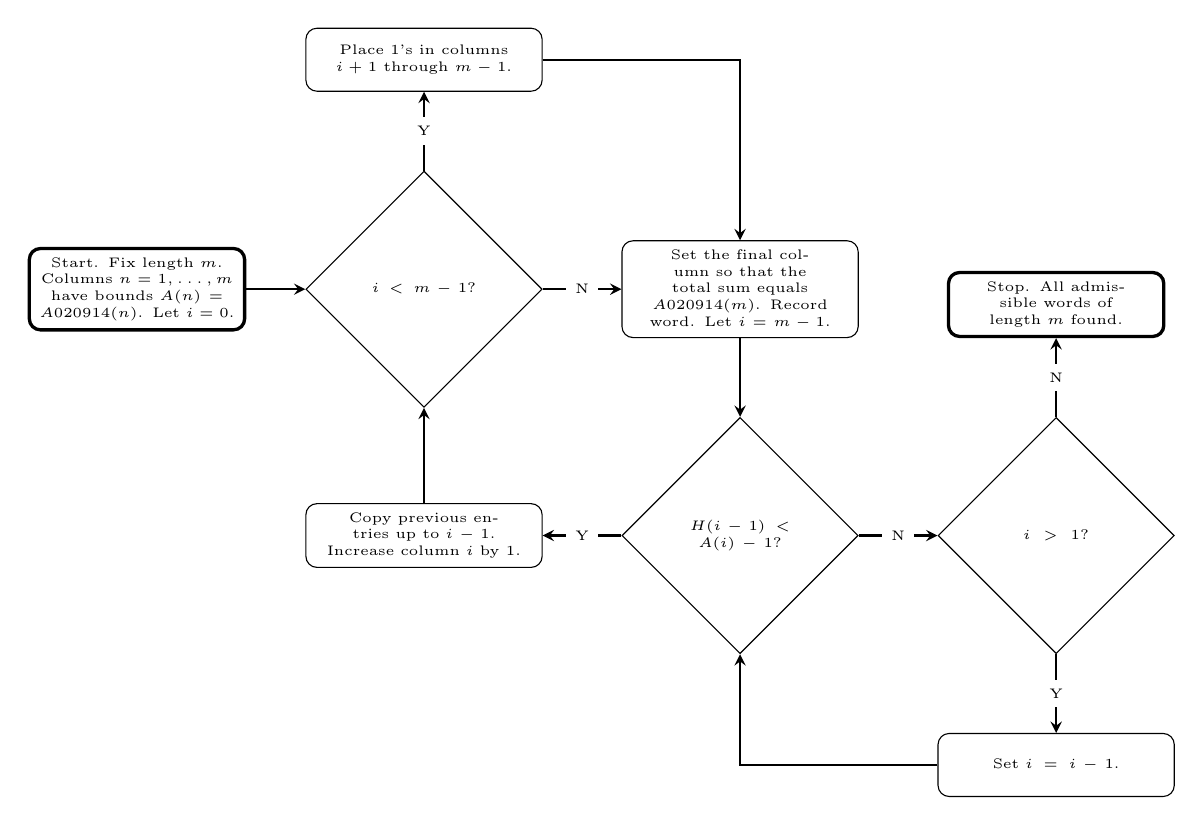
\begin{tikzpicture}[node distance=0.75cm, font=\tiny]

\node(start)        [startstop]                          {Start. Fix length $m$. Columns $n=1,\dots,m$ have bounds $A(n)=A020914(n)$. Let $i=0$.};
\node(test1)        [decision, right=of start]           {$i<m-1$?};
\node(fillones)     [action, above=1.0cm of test1]       {Place 1's in columns $i+1$ through $m-1$.};
\node(lastcol)      [action, right=1.0cm of test1]       {Set the final column so that the total sum equals $A020914(m)$. Record word. Let $i=m-1$.};
\node(test2)        [decision, below=1.0cm of lastcol]   {$H(i-1)<A(i)-1$?};
\node(increment)    [action, left=1.0cm of test2]        {Copy previous entries up to $i-1$. Increase column $i$ by 1.};
\node(test3)        [decision, right=1.0cm of test2]     {$i>1$?};
\node(deci)         [action, below=1.0cm of test3]       {Set $i=i-1$.};
\node(stop)         [startstop, above=1.0cm of test3]    {Stop. All admissible words of length $m$ found.};

\draw [arrow] (start)   -- (test1);
\draw [arrow] (test1)   -- node[fill=white]{Y} (fillones);
\draw [arrow] (test1)   -- node[fill=white]{N} (lastcol);
\draw [arrow] (fillones) -| (lastcol);
\draw [arrow] (lastcol) -- (test2);
\draw [arrow] (test2)   -- node[fill=white]{Y} (increment);
\draw [arrow] (test2)   -- node[fill=white]{N} (test3);
\draw [arrow] (increment) -- (test1);
\draw [arrow] (test3)   -- node[fill=white]{Y} (deci);
\draw [arrow] (deci)    -| (test2);
\draw [arrow] (test3)   -- node[fill=white]{N} (stop);

\end{tikzpicture}
\end{center}
\end{figure}

\subsection*{Example: Words of Length $m=5$}

For $m=5$, the bounds are
\[
A020914(1{:}5) = (2,4,5,7,8).
\]
All admissible parity words must satisfy
\[
H(0)<2,\; H(1)<4,\; H(2)<5,\; H(3)<7,\; H(4)=8.
\]

The search procedure yields the seven admissible words shown in
Table~\ref{tab:m5-words}.

\begin{table}[h]
\centering
\caption{Admissible parity words of length $m=5$.}
\label{tab:m5-words}
\begin{tabular}{c|ccccc}
\textbf{Word} & $d_0$ & $d_1$ & $d_2$ & $d_3$ & $d_4$ \\ \hline
1 & 1 & 1 & 1 & 1 & 4 \\
2 & 1 & 1 & 1 & 2 & 3 \\
3 & 1 & 1 & 1 & 3 & 2 \\
4 & 1 & 1 & 2 & 1 & 3 \\
5 & 1 & 1 & 2 & 2 & 2 \\
6 & 1 & 2 & 1 & 1 & 3 \\
7 & 1 & 2 & 1 & 2 & 2 \\
\end{tabular}
\end{table}

Thus $A186009(m+1)=7$ counts admissible parity words of length $m=5$.  
The final word $(1,2,1,2,2)$ is extremal in the sense that its prefix sums
approach the bounds $A020914(i+1)$ as closely as possible for $i<m-1$
while remaining admissible, and achieve equality at $i=m-1$.

\subsection*{Purpose of This Appendix}

This construction shows that the admissible parity language is generated by a
finite, bounded prefix-sum search governed by \OEIS{A020914}. It provides a
concrete mechanism underlying the horizontal-sum dynamics and explains the
enumeration encoded by \OEIS{A186009}.


\newpage
\section{A Binomial Lower Comparison for \OEIS{A186009}}
\label{app:A047749-lower-bound}

The sequence \OEIS{A047749} admits a horizontal-sum construction analogous to that
of \OEIS{A186009}, but with a stricter terminal rule: its doubling mechanism is
governed by \OEIS{A000034}$(n-2)$ rather than \OEIS{A022921}. As a result,
\OEIS{A047749} forbids \emph{consecutive} doublings, while such events occur
periodically in \OEIS{A186009}. This structural restriction yields a natural
comparison sequence.

\subsection*{Pointwise comparison}

Because \OEIS{A047749} evolves under the same Pascal-type recursion but with a
subset of the admissible doubling events, its row sums form a pointwise lower
bound (up to index shift):
\[
A047749(n) \le A186009(n+1), \qquad n \ge 0.
\]
The two sequences agree initially, but diverge once the first consecutive
doubling occurs in \OEIS{A186009}; thereafter the inequality is strict.

\subsection*{Closed form for \OEIS{A047749}}

Unlike \OEIS{A186009}, the restricted doubling grammar of \OEIS{A047749}
permits an exact description. Its terms split naturally into even and odd
indices:

\paragraph{Even indices ($n=2m$).}
\[
a(n) = \frac{1}{2m+1}\binom{3m}{m}.
\]

\paragraph{Odd indices ($n=2m+1$).}
\[
a(n) = \frac{1}{2m+1}\binom{3m+1}{m+1}.
\]

Equivalently, using Gamma functions,
\[
a(2m)=\frac{\Gamma(3m+1)}{\Gamma(2m+2)\Gamma(m+1)}, \qquad
a(2m+1)=\frac{\Gamma(3m+2)}{\Gamma(2m+2)\Gamma(m+2)}.
\]

\subsection*{Asymptotic growth}

Let $\psi(x)=\Gamma'(x)/\Gamma(x)$ be the digamma function. Differentiating the
logarithm of the Gamma representations gives

\[
\frac{d}{dm}\ln a(2m)
  = 3\psi(3m+1)-2\psi(2m+2)-\psi(m+1),
\]
\[
\frac{d}{dm}\ln a(2m+1)
  = 3\psi(3m+2)-2\psi(2m+2)-\psi(m+2).
\]

Using $\psi(x)=\ln x + O(1/x)$ as $x\to\infty$,
both expressions have the same limit:
\[
\lim_{m\to\infty} \frac{d}{dm}\ln a(n)
= \ln\!\left(\frac{3^3}{2^2}\right)
= \ln\!\left(\frac{27}{4}\right).
\]

Thus
\[
\lim_{n\to\infty}\frac{a(n+2)}{a(n)}=\frac{27}{4},
\qquad
a(n) \sim C\left(\sqrt{\frac{27}{4}}\right)^n.
\]

\subsection*{Implication for \OEIS{A186009}}

Since \OEIS{A047749} is generated by a subset of the admissible doubling events
for \OEIS{A186009}, it provides a constructive comparison sequence with
explicit exponential growth rate
\[
\sqrt{\frac{27}{4}}.
\]
Hence \OEIS{A186009} grows at least exponentially, and strictly faster once
consecutive doubling regimes become active.


\clearpage
\bibliographystyle{unsrtnat}
\bibliography{src/latex/references}

\end{document}  
